Located at the \gls{cern} near Geneva, Switzerland, the Large Hadron Collider (LHC) \cite{2008.LHC} is a circular particle accelerator made up of 27 kilometers of superconducting magnets and RF cavities a hundred meters beneath the Franco-Swiss countryside.
The \lhc~ is fed by a series of smaller accelerators, each subsequent accelerator increasing the energy of the particles by an order of magnitude or more.
This impressive complex of accelerators is shown in Figure \ref{fig:detector:lhc}.
A small bottle of hydrogen feeds a small fraction of its contents into a Duoplasmatron which ionizes the hydrogen into its constituent protons and electrons.
The protons are then injected in Linac2 where they reach 50~\MeV.
Next they are passed on into the Booster, the Proton Synchrotron, and then the Super Proton Synchrotron, which accelerate the protons to an energy of 1.4~\GeV, 25~\GeV, and 450~\GeV respectively.
Finally they enter the \lhc\ where the adjacent oppositely moving beams of protons are each accelerated to the highest energy of 6.5~\TeV (99.9999991\% the speed of light).
The parallel beams meet at four crossing points along the \lhc.
The protons collide at these points with a center-of-mass energy of \rts\ = 13~\tev.
The actual operation energies were 7~\TeV (2010-2011) and 8~\TeV (2012) during Run-1, and 13~\TeV during Run-2.
The four independent physics experiments, \gls{alice}\cite{ALICE:2008ngc}, \gls{atlas}\cite{PERF-2007-01}, the \gls{cms}\cite{CMS:2008xjf}, and the \gls{lhcb}\cite{LHCb:2008vvz} exist at each collision point as seen in Figure \ref{fig:detector:lhc}.
\begin{figure}[h]
  \begin{center}
    \includegraphics[width=0.98\textwidth]{figs/detector/acccomplex.png}
  \end{center}
  \caption[Accelerator complex at CERN]
          {Accelerator complex at CERN~\cite{Mobs:2197559}}
  \label{fig:detector:lhc}
\end{figure}

\subsection{Magnets}
There are two primary types of magnets, the dipoles (bending magnets) and the quadrupoles (squeezing magnets).
The 27~km \lhc\ ring is filled with 1232 15 m long main superconducting dipole magnets and 392 main super conducting quadrupole magnets which bend and focus the the beam around the collider.
With an additional 6000 correcting magnets proton beams are able to be steered in stable circular trajectory.
The standard dipole cross-section schematic is shown in Figure \ref{fig:detector:dipolecrossxsec}, detailing the anatomy of the dipole.
Focusing in on the superconducting coils in Figure \ref{fig:detector:dipolefield}, note there are two dipoles with magnetic fields in opposite directions.
We can easily observe via the familiar right hand rule of the magnetic force law ($F=qv\times B$) that the oppositely circulating proton beams will be bent in the same direction in their path around the LHC ring.
\begin{figure}[ht]
    \centering
    \begin{subfigure}[b]{0.65\textwidth}
      \centering
      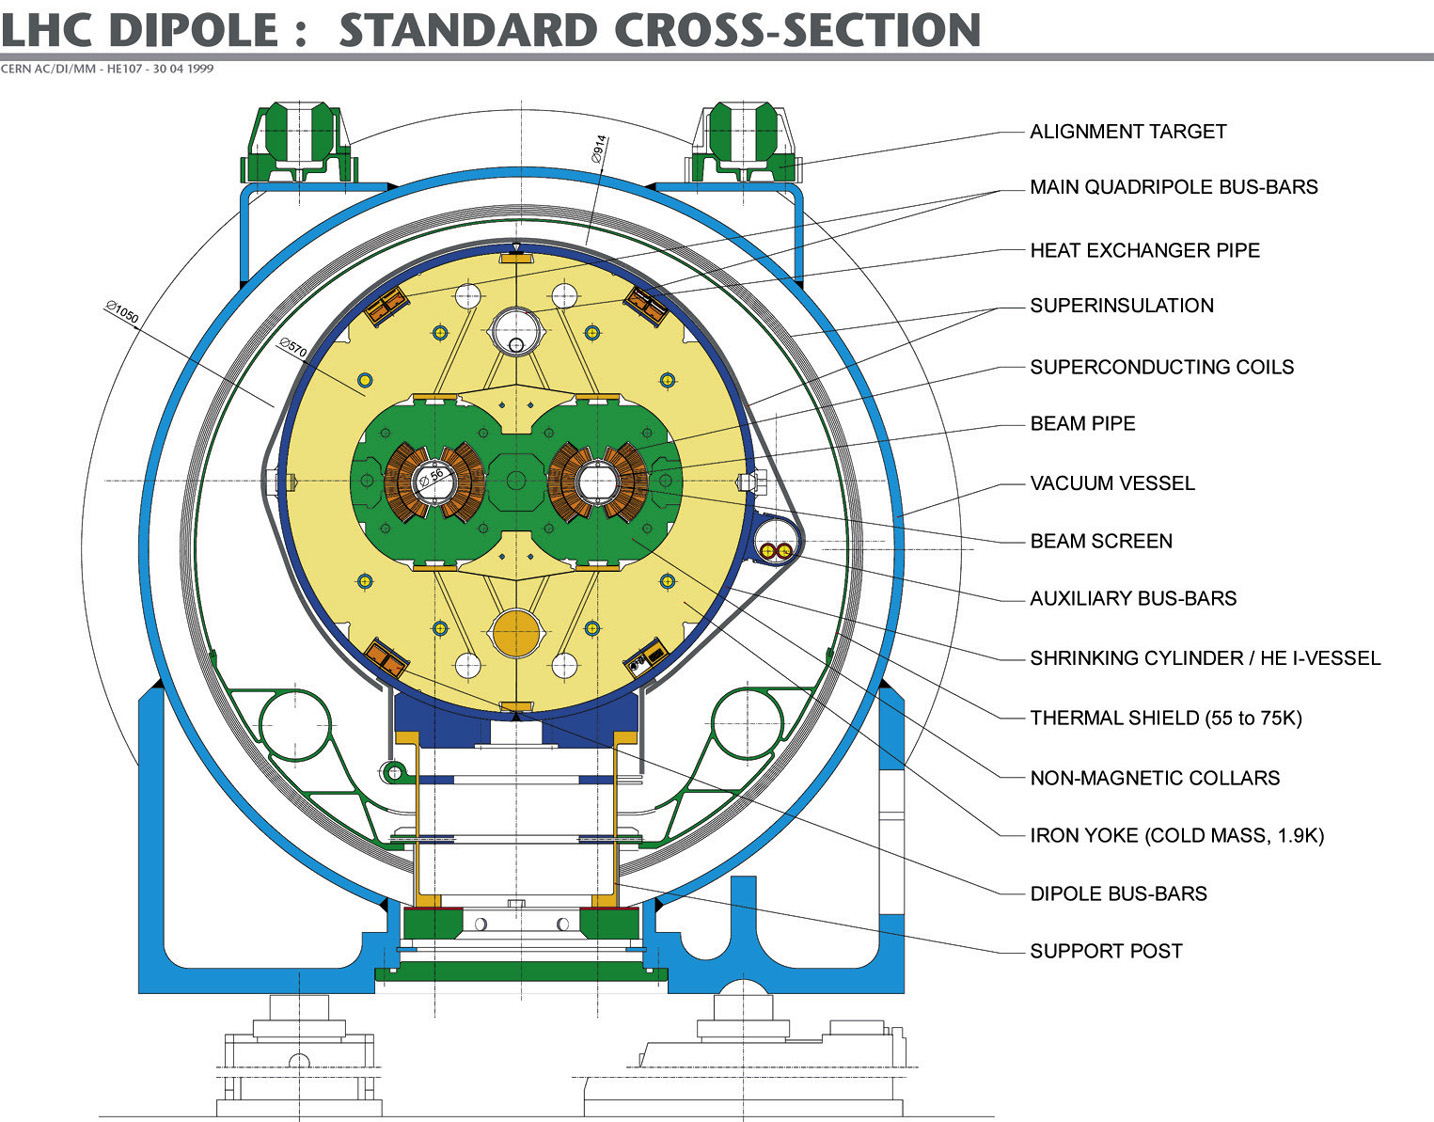
\includegraphics[width=1.0\textwidth]{figs/detector/dipolecrosssection.png}
      \caption{}
      \label{fig:detector:dipolecrossxsec}
    \end{subfigure}
    \hfill
    \begin{subfigure}[b]{0.34\textwidth}
      \centering
      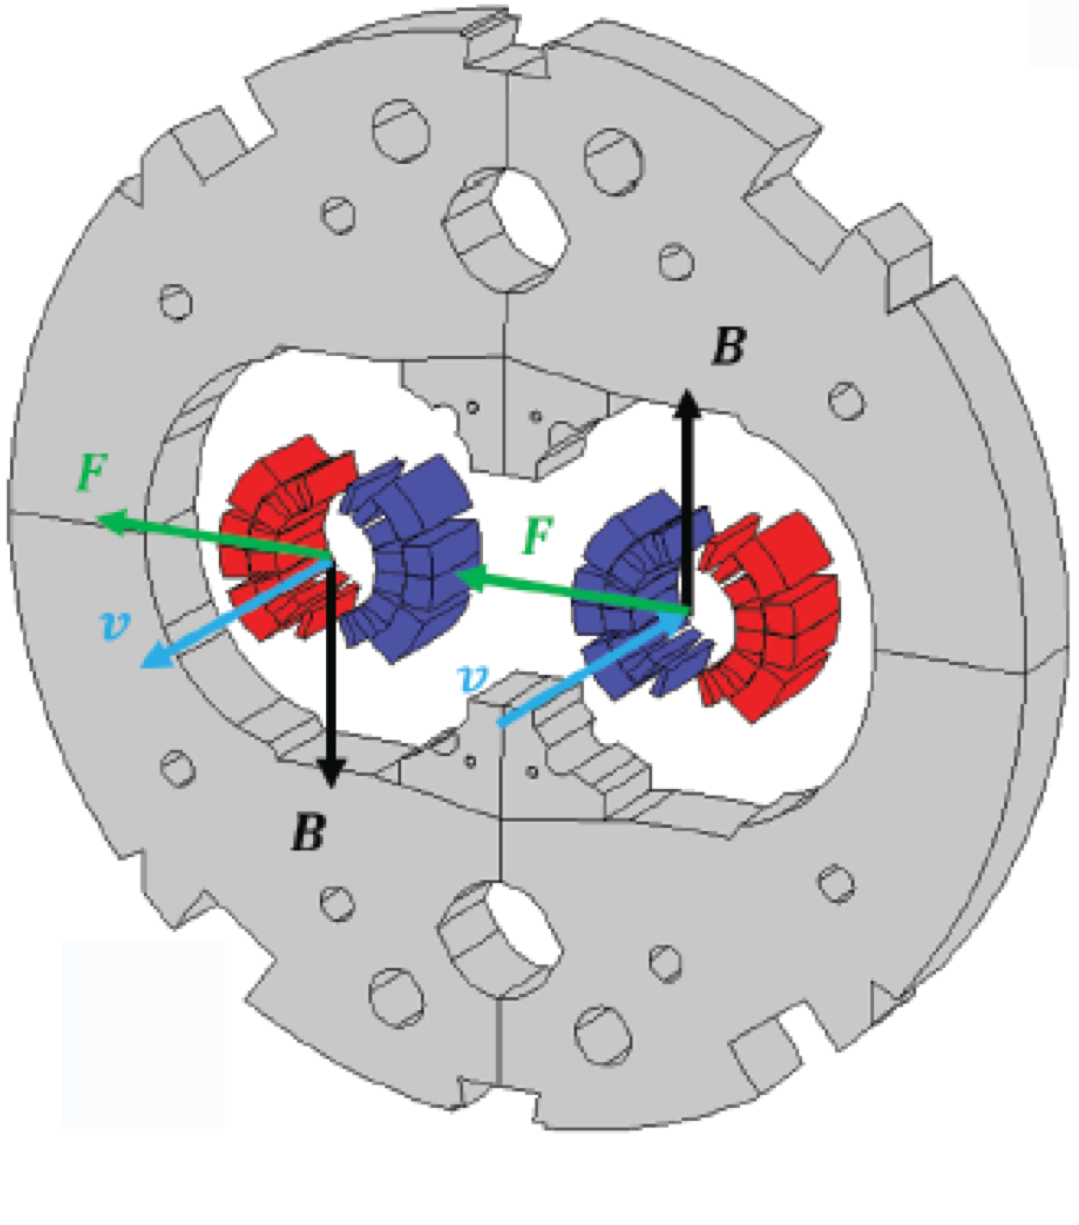
\includegraphics[width=1.0\textwidth]{figs/detector/dipole.png}
      \caption{}
      \label{fig:detector:dipolefield}
    \end{subfigure}
  \caption[Diagram showing the cross-section of an LHC dipole magnet.]
          {(a) Diagram showing the cross-section of an LHC dipole magnet with cold mass and vacuum chamber and (b) the polarity of the magnets with force diagrams depicting how oppositely same charges particles would be bent into the same circle \cite{Team:40524}\cite{Dipole}.}
      \label{fig:detector:dipole}
\end{figure}
The quadrupole magnet cross-section is effectively identical to the dipole only now with a swap of the dipole superconducting coil configuration with that of the quadrupole configuration shown in Figure~\ref{fig:detector:quadrupole}.
\begin{figure}[ht]
  \begin{center}
    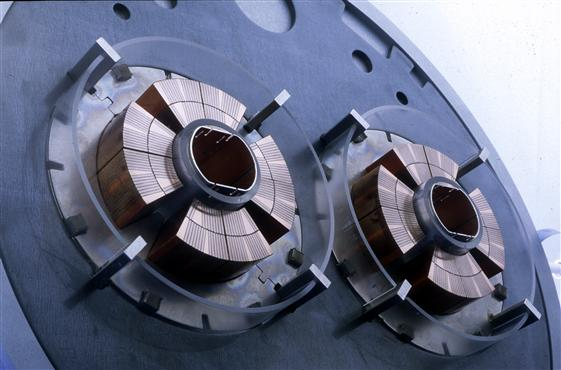
\includegraphics[width=0.58\textwidth]{figs/detector/quadrupole.png}
  \end{center}
  \caption[Cross-section of a model of the superconducting quadrupole magnet]{Cross-section of a model of the superconducting quadrupole magnet~\cite{Laurent:40918}}
  \label{fig:detector:quadrupole}
\end{figure}
The last set of magnets required are the low-$\beta$ triplets, so-called due to their three quadrupole system that is used to focus the beams, and that it is the triplet's job to minimize the $\beta$-function, which is proportional to beam size, are located on either side of each of the four experiments.
This system does a final squeeze on the beams, making them 12.5 times narrower – from 0.2 millimeters down to 16 micrometers across, all the while simultaneously crossing the opposing beams at the center of the detectors.
Figure \ref{fig:detector:beamcross} illustrates these low-$\beta$ triplets at work as the beam sizes are drastically reduced in the last 60~m on each side of the interaction point.
After colliding, the particle beams are separated again by dipole magnets.
\begin{figure}[ht]
  \begin{center}
    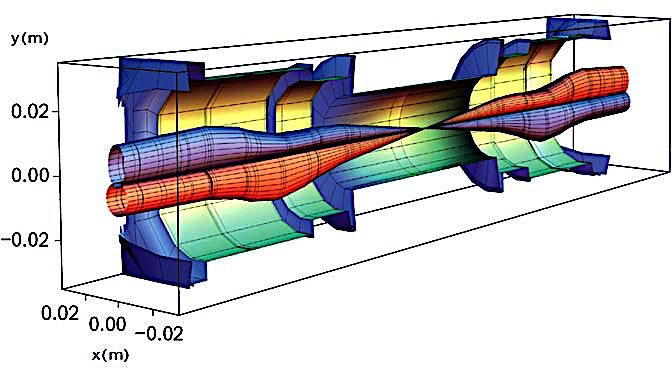
\includegraphics[width=0.98\textwidth]{figs/detector/beamcross.png}
  \end{center}
  \caption[Beam envelopes in the interaction region around point 1 (\ATLAS) showing how the beam sizes are reduced in the last 60 m on each side of the interaction point following the squeeze.]{Beam envelopes in the interaction region around point 1 (\ATLAS) showing how the beam sizes are reduced in the last 60 m on each side of the interaction point following the squeeze.
  Note the different transverse scale: the radius of the cut-away beam pipe is just 18 mm at the collision point.
  The clockwise beam is in blue and the anti-clockwise beam is in red~\cite{BeamEnvelopes}}
  \label{fig:detector:beamcross}
\end{figure}

\subsection{Beams, Buckets, and Bunches}
\label{sec:detector:beamsbucketsbunches}
The proton beam structure consists of the base unit known as a ``bunch'' where each bunch is on the order of $10^{11}$ protons.
A bunch is a direct consequence of the harmonics of the RF cavities.
Given the revolution frequency of the protons and RF frequency the \lhc~has a total of 35640 harmonics.
Each one of these harmonics is known as a ``bucket'' and is effectively a potential well for the protons in which a bunch \emph{can} exist.
So while in principle the \lhc\ could accelerate 35640 bunches at a time per beam, practically this would result in a bunch spacing of 2.5~ns and the \lhc's diverting magnets would not have enough time to trigger and execute a beam dump (never mind the fact that it would make data taking an incredible challenge as it would light up our detectors like a Christmas tree even if we could!).
These technical restrictions give rise to the nominal proton beam at the \lhc\ made up of 2808 bunches with 25~ns spacing (10 empty buckets spacing). 
Figure~\ref{fig:detector:bunch} shows a more detailed schematic of the 25~ns bunch structure.
This amounts to $ 2808~\text{bunches} ~\times~ 10^{11} ~\text{protons} = 3\cdot10^{14}~\text{protons/beam}$, or $6\cdot10^{14} ~\text{protons}$ for the two beams.
\begin{figure}[ht]
  \begin{center}
    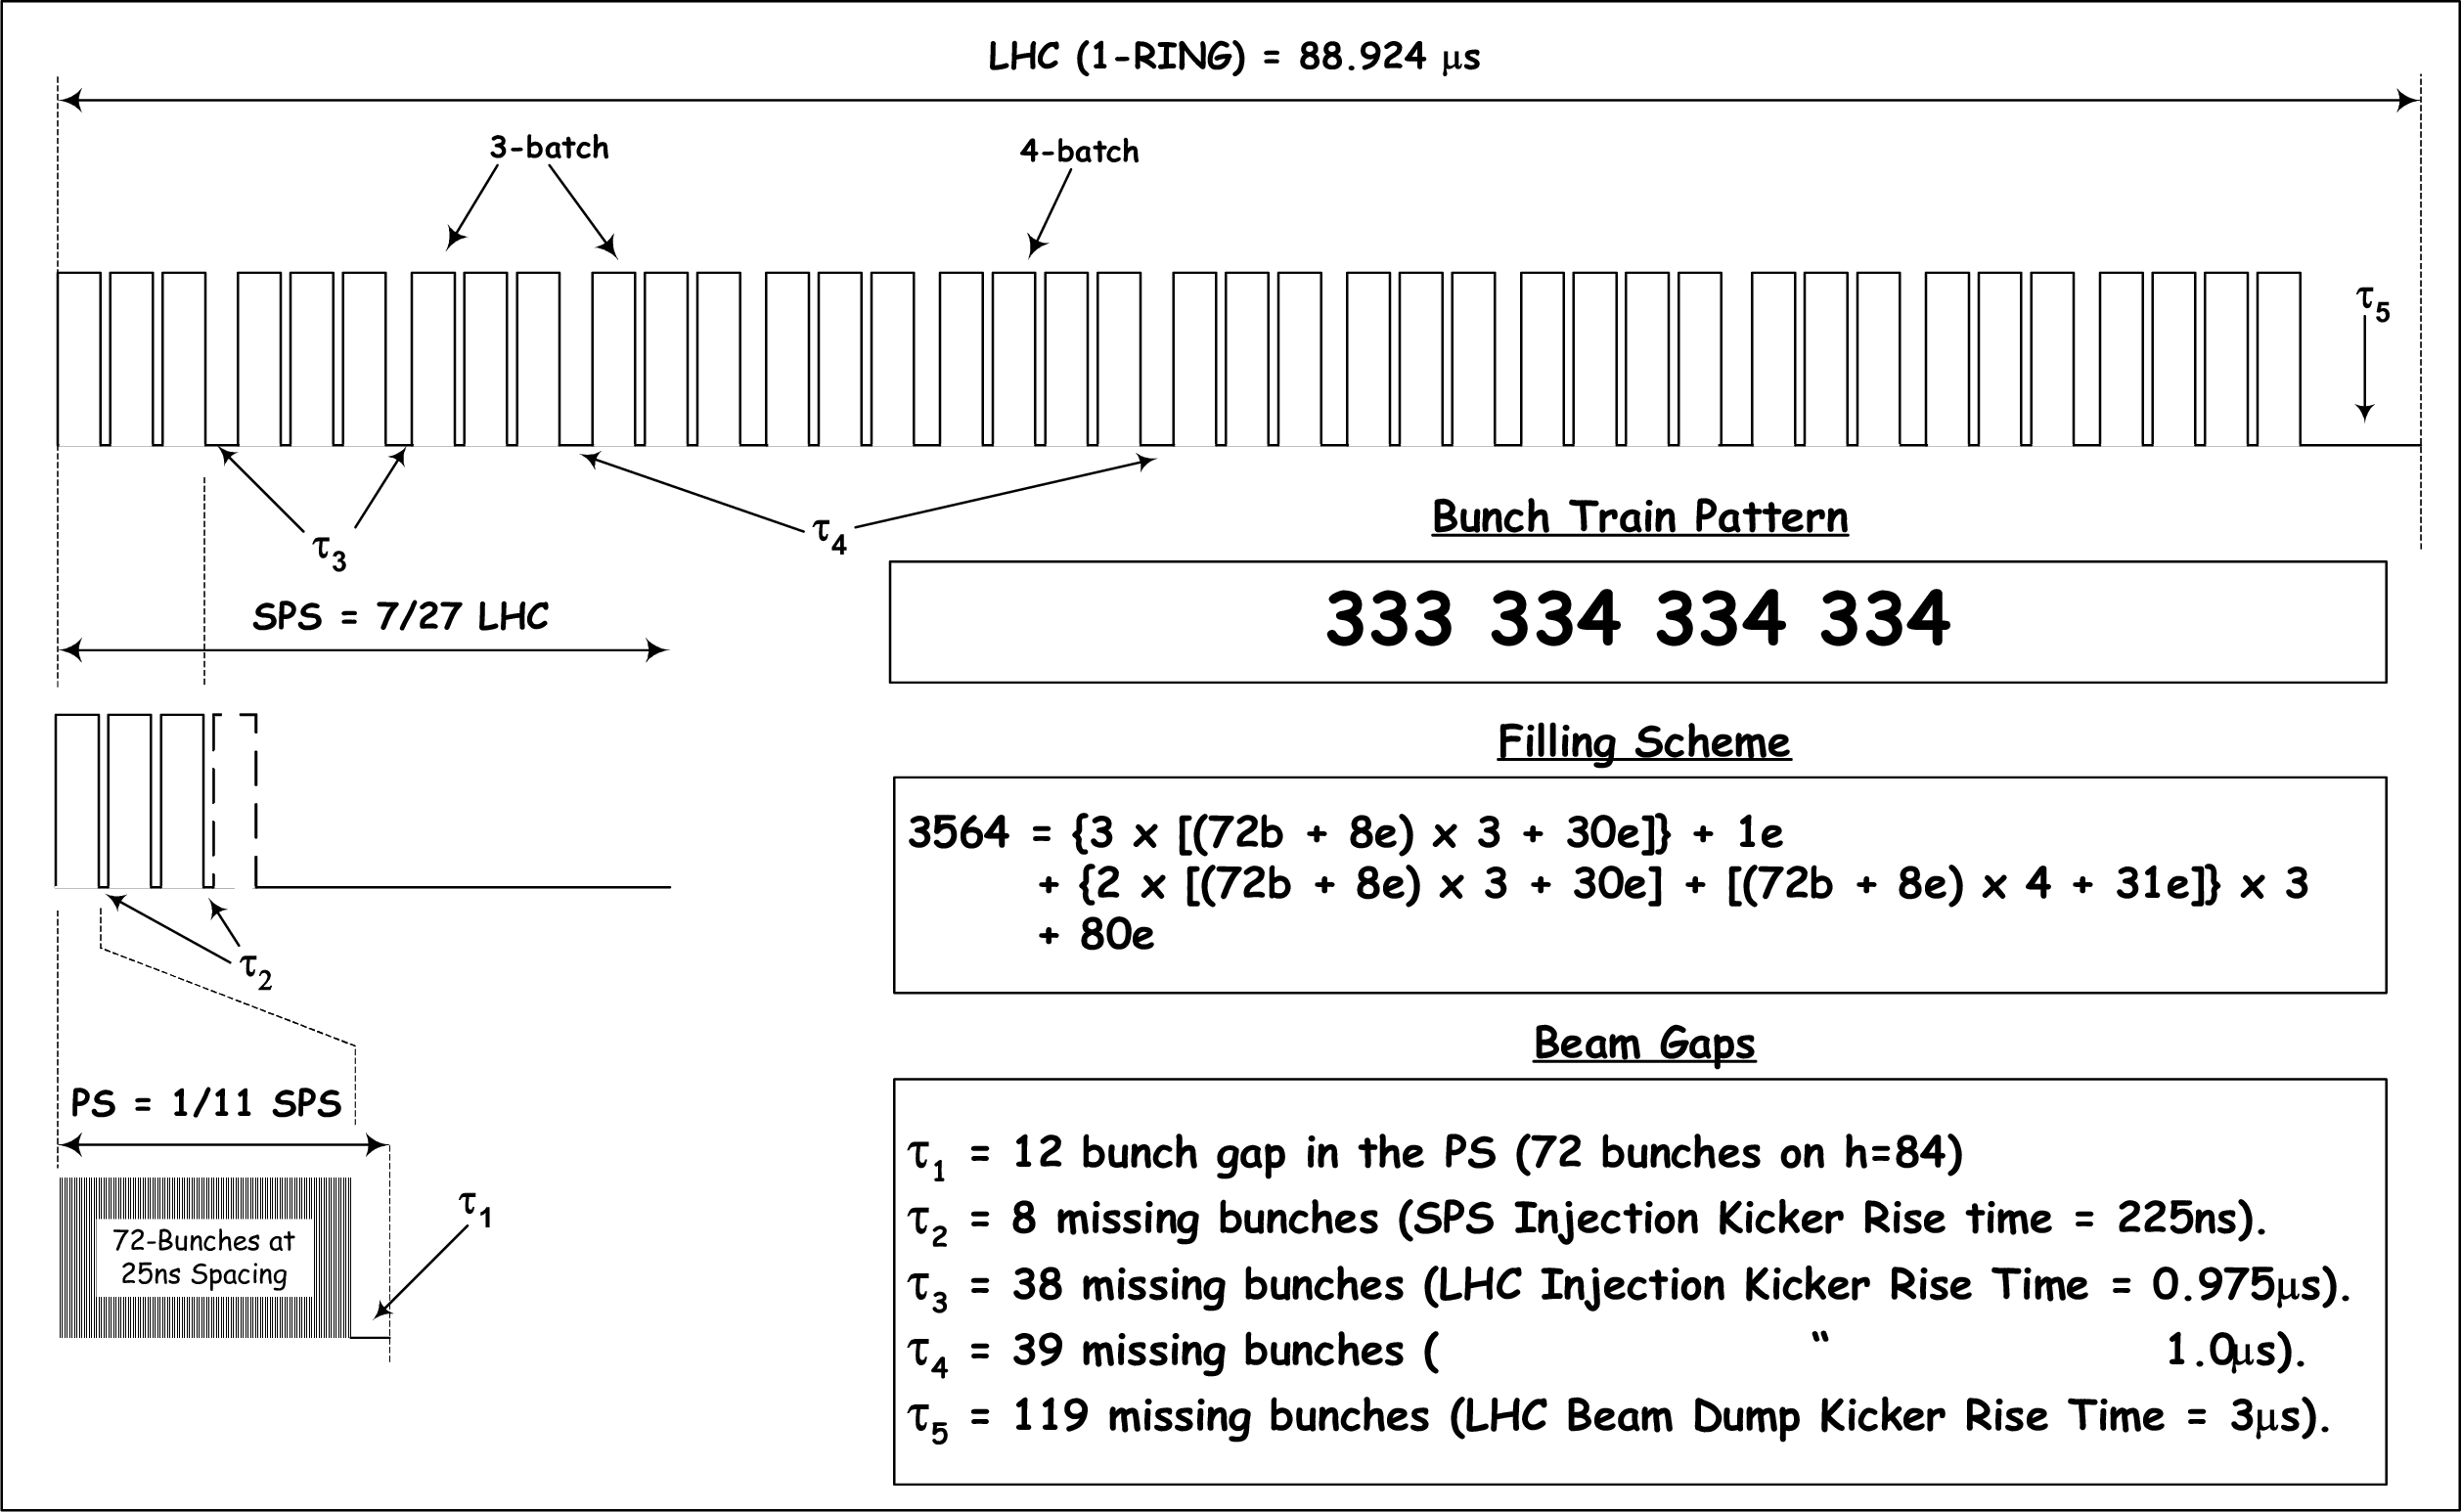
\includegraphics[width=0.98\textwidth]{figs/detector/bunch_structure.png}
  \end{center}
  \caption[Schematic of the Bunch Disposition around an LHC Ring for the 25~ns Filling Scheme]{Schematic of the Bunch Disposition around an LHC Ring for the 25~ns Filling Scheme. 
  We can recover the quoted number of bunches of 2808 in the text by sending the number of missing bunches, denoted with an ``$e$'' to zero ($e \rightarrow 0$) in the ``Filling Scheme'' calculation.
  Or equivalently adding up all the integers present in ``Bunch Train Pattern'' and multiplying by 72. \cite{Bailey:691782} }
  \label{fig:detector:bunch}
\end{figure}
From September 2017 to the end of data-taking in 2017 this structure was modified to the ``8 bunches'' and ``4 empty (slots)'' spacing in order to mitigate excessive beam dumps caused by frozen particles of gas being detached from the inside of the beam pipe during a run.
This resulted in a decrease of the number of bunches to 1920 but an actual \emph{increase} in activity in the detector by the measure of the mean number of interactions per bunch crossing, $\langle \mu \rangle$.  
Where $\langle \mu \rangle$ corresponds to the mean of the Poisson distribution of the number of interactions per crossing calculated for each bunch.
This is calculated from the instantaneous per bunch luminosity as $\mu$=$L_{bunch}\times \sigma_{inel} / f_{r}$ where $L_{bunch}$ is the per bunch instantaneous luminosity, $\sigma_{inel}$ is the inelastic cross section which is taken to be 80 mb for 13~\TeV collisions, and $f_{r}$ is the LHC revolution frequency.
This bunch structure change was reflected in standard luminosity vs. $\langle \mu \rangle$ plot in Figure \ref{fig:detector:pileupprofile} as the infamous ``double-hump'' (Bactrian?) year in purple.
Each fill of the LHC with two proton beams last for 10 hours with stable beam conditions, i.e. a fill corresponds to a  productive physics data collection period before the beam is depleted to the point that the bunch density becomes low enough that it becomes more favorable to dump the beam and re-fill for another run than to continue the current run.

\subsection{Pileup}\label{sec:detector:pileup}
The number of interactions per bunch crossing is not only an important measure for data yield but also for the activity present in the detectors, as it directly influences physics analyses at almost every level. 
If the \lhc\ were to be filled such that $\langle \mu \rangle$ = 1 we would of course have very clean and straight forward detector signatures and this discussion would be moot.
However the vast majority of potentially accessible processes at the \lhc\ would be practically unattainable due to their extreme rarity, so the high rate of proton collisions is essential for modern collider particle physics analyses and the handling of many interactions is necessary.
This additional activity to be handled is refered to as ``pileup.'' 
\begin{figure}[tbp]
  \begin{center}
    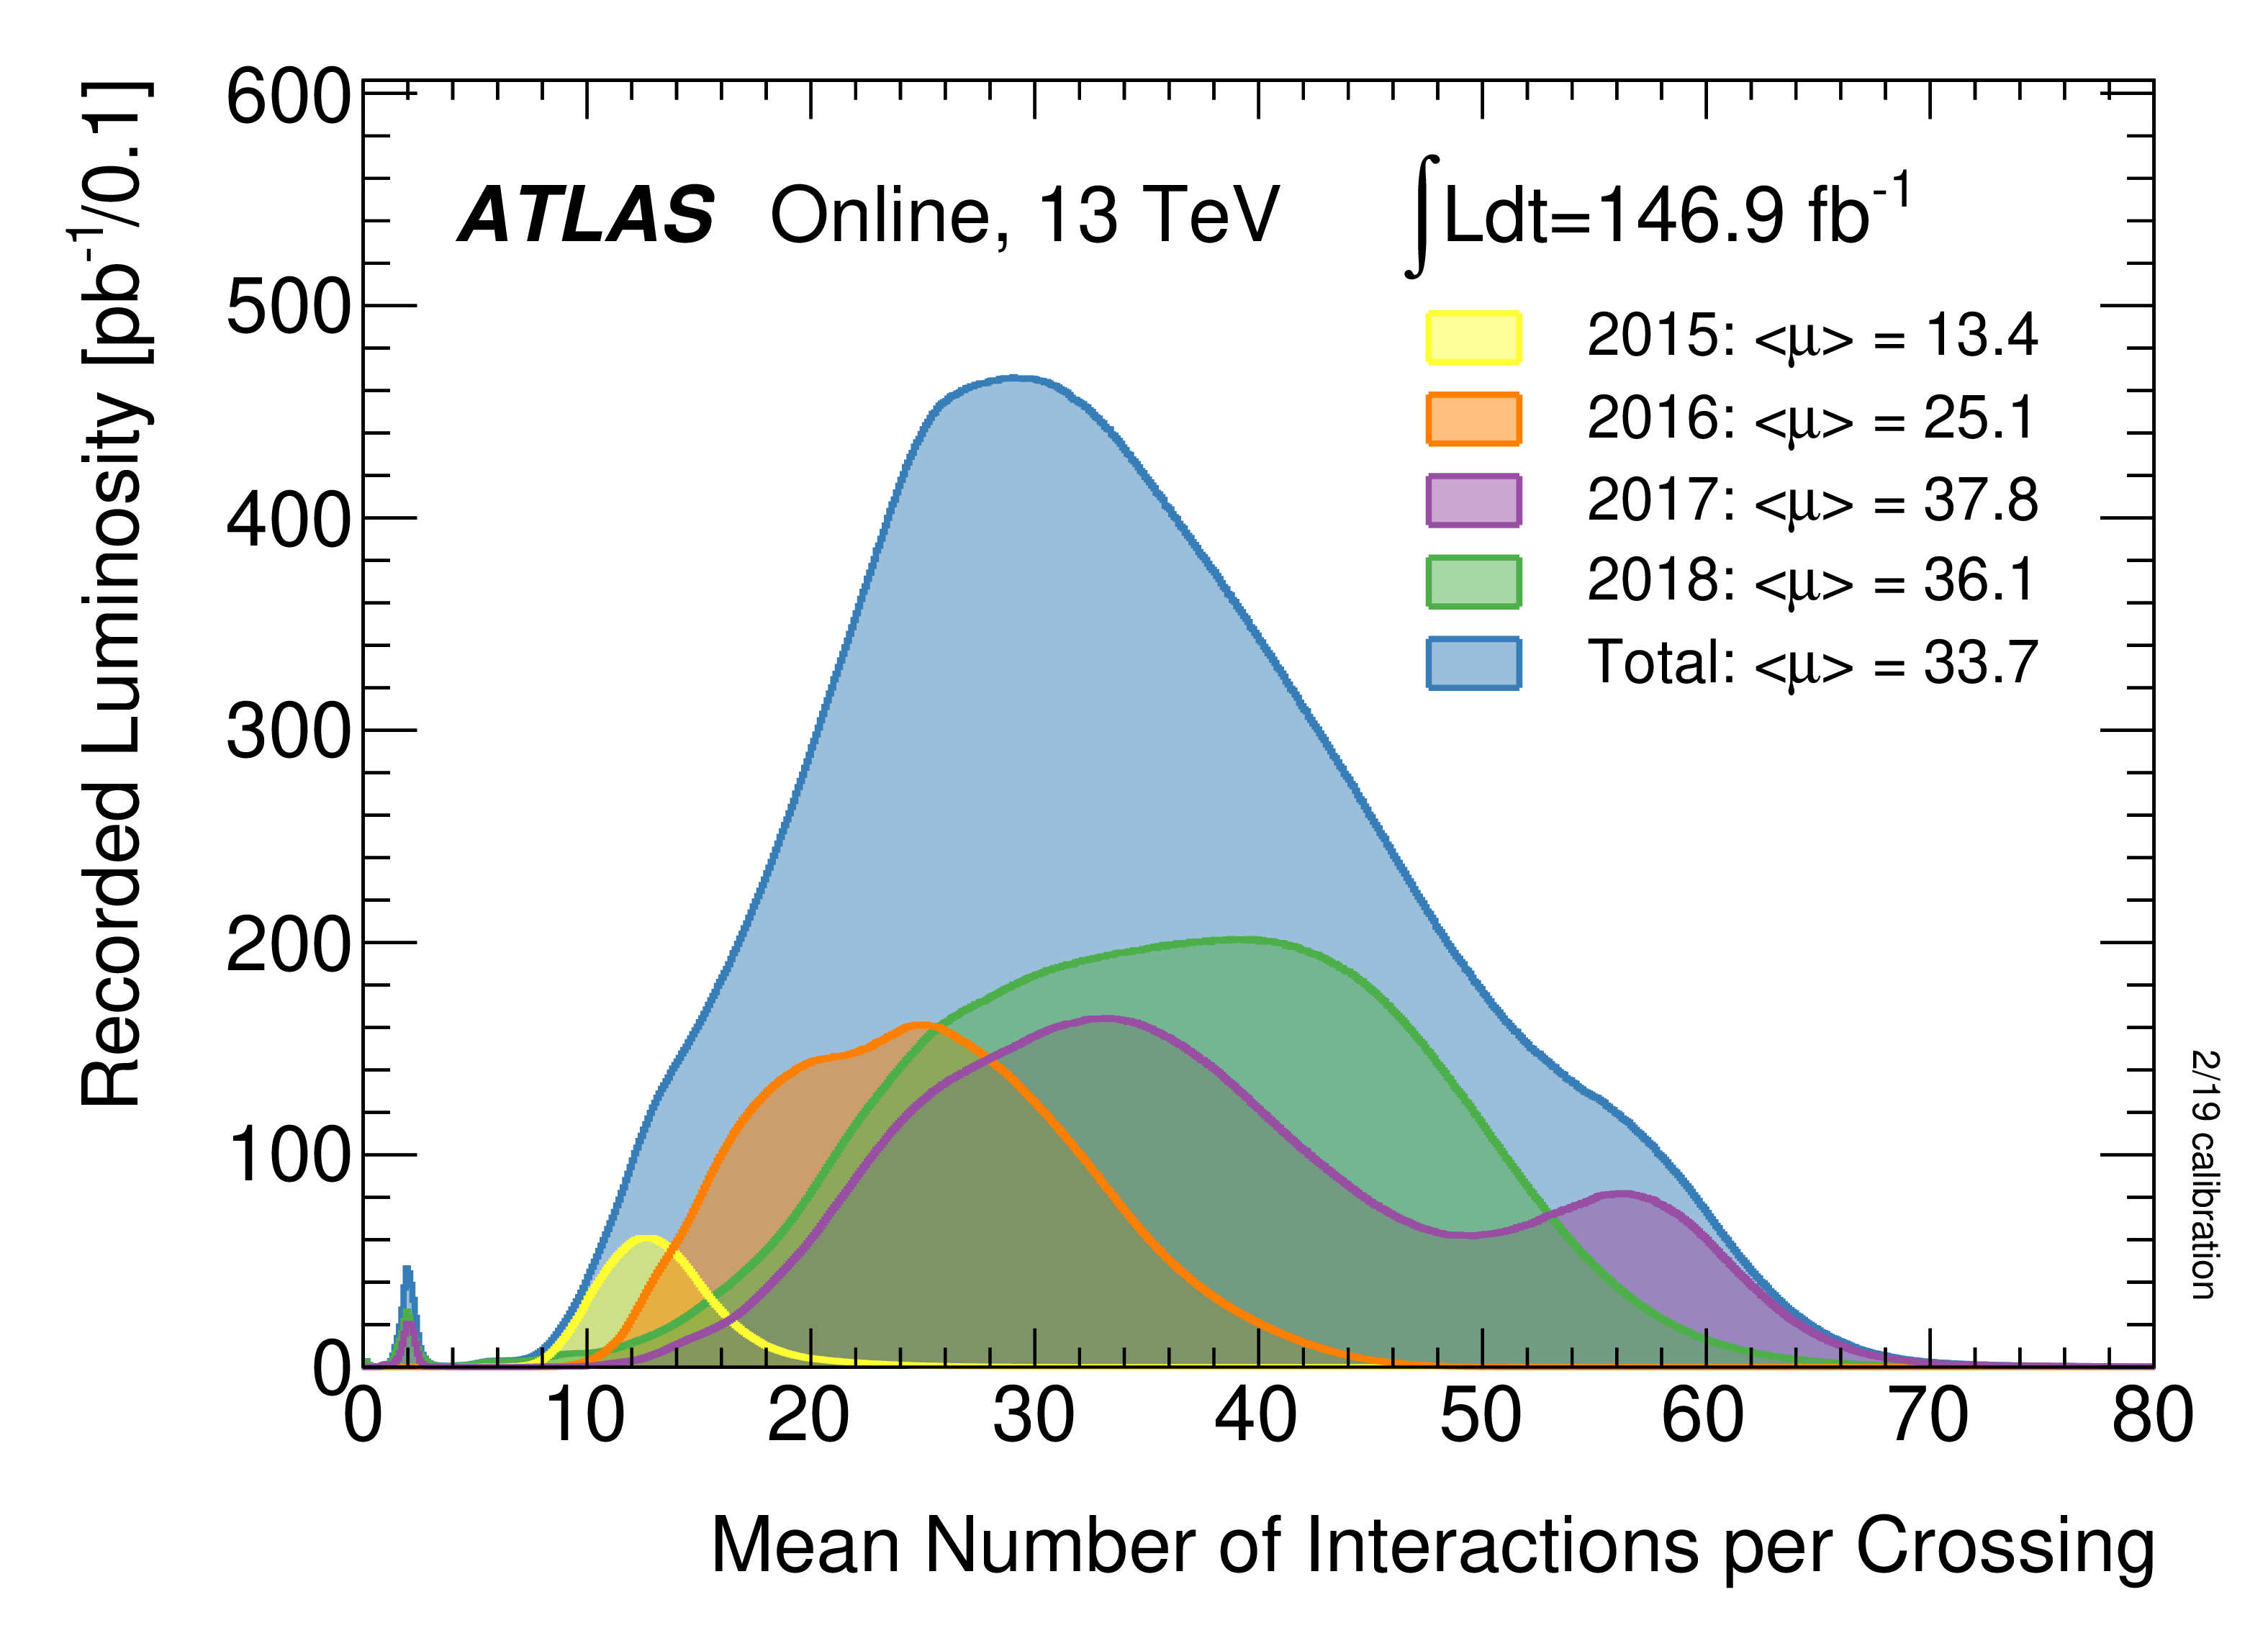
\includegraphics[width=0.88\textwidth]{figs/detector/pileupprofile.png}
  \end{center}
  \caption[The luminosity-weighted distribution of the mean number of interactions per crossing for 2015-2018 pp collision data at 13 TeV centre-of-mass energy.]
          {Shown is the luminosity-weighted distribution of the mean number of interactions per crossing for 2015-2018 pp collision data at 13 TeV centre-of-mass energy.
          All data recorded by ATLAS during stable beams is shown, and the integrated luminosity and the mean $\mu$ value are given in the figure.
          The luminosity shown represents the preliminary 13 TeV luminosity calibration for 2018, released in February 2019, that is based on van-der-Meer beam-separation scans \cite{MeanMuLuminosity}.}
  \label{fig:detector:pileupprofile}
\end{figure}
Figures \ref{fig:detector:pileup25} and \ref{fig:detector:pileup65} show \ATLAS\ event displays for events with 25 and 66 reconstructed vertices, respectively, to demonstrate what these high pileup collisions look like in the \ATLAS\ detector.
So as one can easily imagine from these figures high pileup environments pose experimental difficulties for the detectors as the interaction of interest must be distinguished from all the other simultaneous collisions. 
\begin{figure}[h]
  \begin{center}
    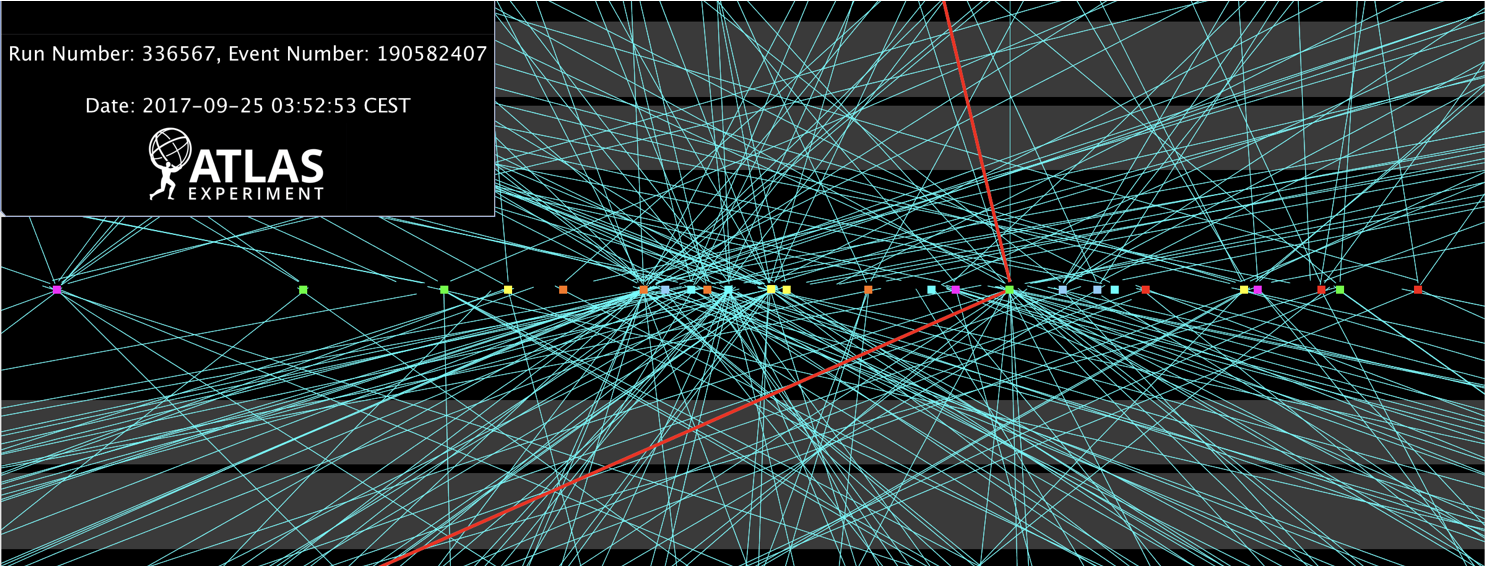
\includegraphics[width=0.98\textwidth]{figs/detector/pileup25.png}
  \end{center}
  \caption[A Z candidate is reconstructed in a beam crossing with 24 additionally reconstructed vertices from minimum bias interactions.]
          {A display of a $Z\rightarrow \mu\mu$ candidate event from proton-proton collisions recorded by \ATLAS\ with LHC stable beams at a collision energy of 13~\TeV.
          The Z candidate is reconstructed in a beam crossing with 24 additionally reconstructed vertices from minimum bias interactions.
          The hard interaction vertex is represented by a green square from which the two muons (red tracks) are emerging. Tracks with \pt\ $> 500$~\MeV are displayed ~\cite{Pileup25}.}
  \label{fig:detector:pileup25}
\end{figure}
\begin{figure}[h]
  \begin{center}
    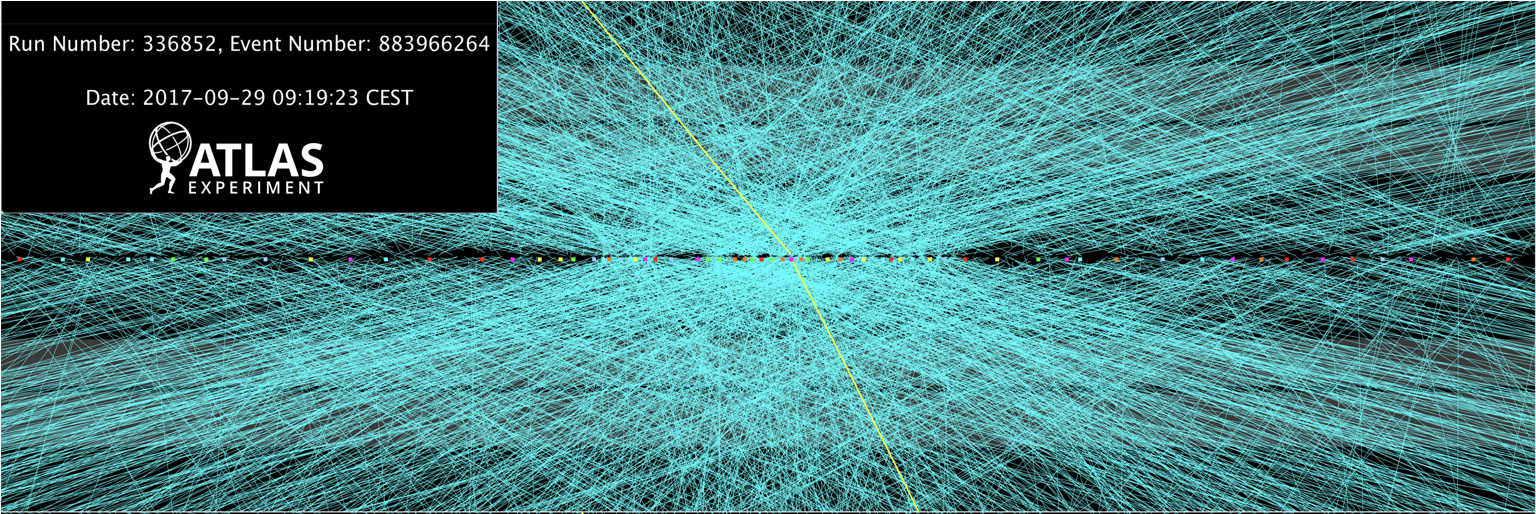
\includegraphics[width=0.98\textwidth]{figs/detector/pileup65.png}
  \end{center}
  \caption[A Z boson candidate is reconstructed in a beam crossing with 65 additionally reconstructed vertices from minimum bias interactions]
          {A display of a $Z\rightarrow \mu\mu$ candidate event from proton-proton collisions recorded by ATLAS with LHC stable beams at a collision energy of 13~\TeV. The Z boson candidate is reconstructed in a beam crossing with 65 additionally reconstructed vertices from minimum bias interactions.
          The figure shows tracks with a cut on track \pt\ of 100~\MeV~\cite{Pileup65}.}
  \label{fig:detector:pileup65}
\end{figure}





